\subsection{Storm [SP]}

Batch processing is not applicable for real time computing.
Hadoop, the best known tool for batch processing, is helpless when it is needed to handle streaming data and obtain immediate result.
The main advantage of real time processing, the guaranteed time delay between a request and a result can be broken simply because the waiting time for the next batch is too long.
Therefore new systems, designed for real-time processing, have appeared.
One of such systems is an open source project named \textit{Storm}.

Storm is a \textit{complex event-processing} (CEP) system.
Complex event processing means gathering data from different sources, combining it and making conclusions from it.
For example, such system keeps track of significant changes in traffic reports or stock market feeds and immediately responds to them. 

Storm is implemented in a dialect of the Lisp language named Clojure.
Clojure is a functional language like Lisp, but it also supports multithreaded programming.
Clojure runs on the Java Virtual Machine, however applications within Storm can be written in Java, Scala, JRuby, Perl and PHP.
Moreover, one can use a Structured Query Language adapter for streaming data directly into Storm topoloy.

\mnote{Storm architecture}
The Storm cluster has a master node called \textit{Nimbus} and \textit{worker} nodes.
Nimbus assignes tasks for workers and monitors failures.
There is a deamon called \textit{Supervisor} on every worker node.
The supervisor is responsible for starting and stopping worker processes assigned by Nimbus.
ZooKeeper coordinates the interaction between Nimbus and Supervisors.
It stores the state of all the nodes, making the system stable to failures.
If any of the nodes is killed, ZooKeeper immediately restarts it, enhancing Storm cluster stability.
ZooKeeper is described in more details later in this chapter.

The basic concept of Storm is a \textit{topology}.
It is a graph of computation, that shows how data should be processed and passed between the nodes.
One can implement a topology in any programming language, because topology definition is a Thrift structure.
Thrift is a framework that allows to develop cross-language services.	

The data stream consists of an unbounded set of \textit{tuples}.
A tuple can contain both standard data types (integer, float, byte array) as well as user-defined types.
Every stream has its own ID.
The sources of streams called \textit{spouts}. 

The next important Storm primitive is \textit{bolt}.
Figure~\ref{fig:storm_architecture} shows the interaction between spouts and bolts.
The stream of tuples originates from a spout and goes through a sequence of bolts.
Every bolt performs a transformation on incoming data stream, like aggregating, filtering, or interaction with external parts such as databases.
A bolt can receive information from several spouts and stream it to multiple bolts.

\begin{figure}
  \centering
  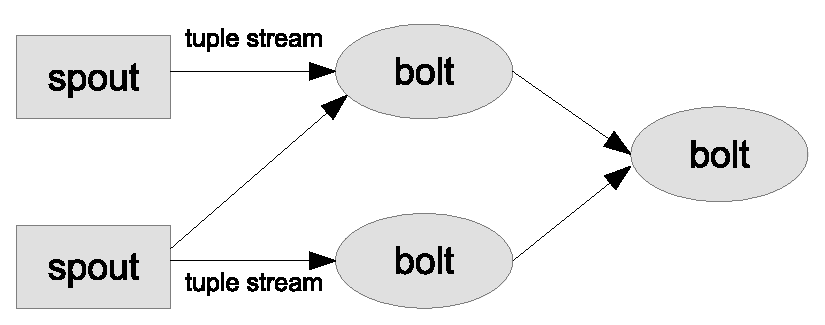
\includegraphics [width=0.5\textwidth]{images/storm_architecture}
  \caption{Storm architecture}
  \label{fig:storm_architecture}
\end{figure}

For example, MapReduce word counting example can be easily implemented with Storm.
Such system counts how many times each word occures in a given input data.
In the case of Storm one needs 
(1) a spout to generate text data, 
(2) one bolt to implement the Map function for word tokenisation and 
(3) one bolt to implement the Reduce function for aggregation the amounts of words occurences. 

Storm allows to group the stream of tuples in different ways.
For instance, shuffle grouping randomly distributes tuples to bolts such as each bolt receives approximately the same number of tuples.
Field grouping partitions tuples according to contained fields.
Also other grouping methods exist, including the custom grouping.

The Listing~\ref{lis:simple_storm_topology} represents a simple topology.

\begin{lstlisting}[caption=Simple Storm topology, label=lis:simple_storm_topology]
java TopologyBuilder builder = new TopologyBuilder();
builder.setSpout("myspout", new TestSpout(), 10);
builder.setBolt("mybolt1", new TestBolt(), 3) .shuffleGrouping("myspout");
builder.setBolt("mybolt2", new TestBolt(), 2) .shuffleGrouping("mybolt1");
\end{lstlisting}

Here topology consists of one spout and two bolts.
The stream of tuples originates from \textit{myspout}, then it is passed to \textit{mybolt1} and finally to \textit{mybolt2}.
In both cases tuples are grupped using the schuffle grouping method.
The integer numbers in \textit{setSpout} and \textit{setBolt} define the amount of parallelism for the node.

The implementation charasteristics of Storm lead to high performance and guaranteed fault tolerance.
It uses ZeroMQ for passing messages between the tasks.
Messages are automatically serialized and deserialized to Storm primitive types.
The usage of this message queue helps to avoid intermediate queueing, thus improving performance.
Furthermore, Storm guarantees the processing of every tuple.
In the case of a fault during message processing, a tuple is replayed from the spout.
There is also a fault detection mechanism on task level, when the failed task is quickly reassigned to restart the processing.
Storm has supervisors to manage the processes, that leads to efficient usage of resources.

Storm cooperates with message queue systems in such a way that every message is fully processed.
It builds a tuple tree, that reflects the motion af all the tuples.
Only when every message in the tuple tree is processed, a tuple is considered to be fully processed.

To give an example, let us take a message queue that supplies a spout with messages.
When the spout takes a message from the queue, the message state changes to 'pending'.
In this state it cannot be sent to other consumers.
Moreover, all the messages in pending state are returned to message queue if their consumer disconnects.
Storm assignes a unique id to the message, if it is not given by the message queue.
Using this id Storm can keep track of this message during processing.
The system receives this message when the \textit{nextTuple} method of the spout is called.
The spout emits the message along with its id to the consuming bolts.
When a tuple is fully processed, the \textit{ack} method of the original spout is called. 
In the case of time-out Storm calls the \textit{fail} method of the same spout.
Only when \textit{ack} or \textit{fail} method is called, the spout sends an ack or fail message to the message queue.
The message queue cancels the pending state of the message, taking it off the queue in the case of success and putting it back otherwise.

Storm can process not only the tuple trees, but also directed acyclic graphs.
It happens when an output tuple is anchored to several input tuples.
\textit{To anchor} means to specify a link in the tuple tree.
Multi-anchored tuples often appear during streaming aggregation or joining.
 
As it was mentioned, Storm tracks every tuple using its unique id.
Additionally, as each tuple exists within a tree, it knows all the tuples ids of this tree.
For example, if a bolt emits a new tuple, this tuple carries the ids of spout tuples received by this bolt along with its own id.
Such storage mechanism is used	because when the tuple is acked or failed, it should inform Storm about its dependencies to restore the state of the tuple tree.  

The acker task is responsible for acking the tuple.
First, Strom stores the mapping between an acker task and a spout tuple id.
As every tuple keeps ids of spout tuples in the tree it exists within, it knows the acker tasks it should communicate with.
A tuple informs an acker task when the tree is fully processed and the tuple is acked.
Second, the acker task should send a complition message to the spout task that emitted this tuple.
For this purpose, on creation of a new tuple a spout task notifies the appropriate acker task that its task id is linked to that spout tuple.

For acker task tracking the huge tuple trees explicitly is not efficient.
Thus Storm uses a special tracking strategy.
An acker task stores a map: on the one side it has a spout tuple id and on the other side a pair of values.
One of the values is a task id the spout tuple originates from, and the other is an 'ack val', the 64 bit number.
The 'ack val' represents the state of the tuple tree without storing it in memory.
This number is a result of XOR operation on all created and acked tuple ids of the tree.
Therefore, when the 'ack val' is equal to zero, it means that the tree is completed.